\documentclass[11pt]{article}
% ---------------------------------------------------------------------------
%  ccint project wrap-up — preamble
%  Compiles with pdfLaTeX (Overleaf default; no configuration needed).
% ---------------------------------------------------------------------------
\usepackage[T1]{fontenc}
\usepackage[utf8]{inputenc}
\usepackage{lmodern}
\usepackage[letterpaper,margin=1in,headheight=14pt]{geometry}
\usepackage{microtype}
\setlength{\emergencystretch}{3em}   % 允许必要时额外伸缩，消除长代码标识符造成的溢出

\usepackage{booktabs}
\usepackage{tabularx}
\usepackage{longtable}
\usepackage{array}
\usepackage{multirow}
\usepackage{amssymb}
\usepackage{amsmath}
\usepackage{enumitem}
\usepackage{fancyhdr}
\usepackage{titlesec}
\usepackage{graphicx}
\graphicspath{{figures/}}
\usepackage{tikz}
\usetikzlibrary{arrows.meta,positioning,calc,fit,backgrounds}
\usepackage[skins,breakable]{tcolorbox}

\usepackage[dvipsnames]{xcolor}
\definecolor{ink}{HTML}{1A1A1A}
\definecolor{accent}{HTML}{1F4E79}
\definecolor{warn}{HTML}{9C4221}
\definecolor{good}{HTML}{22543D}
\definecolor{rule}{HTML}{C8CDD4}
\definecolor{softbg}{HTML}{F4F6F8}
\definecolor{accentbg}{HTML}{EAF0F6}

\usepackage[font=small,labelfont={bf,color=accent},skip=8pt]{caption}

\usepackage[colorlinks=true,linkcolor=accent,urlcolor=accent,citecolor=accent]{hyperref}

% --- headers ---------------------------------------------------------------
\pagestyle{fancy}
\fancyhf{}
\renewcommand{\headrulewidth}{0.4pt}
\fancyhead[L]{\footnotesize\textcolor{accent}{ccint — Canada Cyber Social Intelligence}}
\fancyhead[R]{\footnotesize\thepage}

% --- section styling -------------------------------------------------------
\titleformat{\section}{\Large\bfseries\color{accent}}{\thesection}{0.7em}{}
\titleformat{\subsection}{\large\bfseries\color{ink}}{\thesubsection}{0.6em}{}
\titleformat{\subsubsection}{\normalsize\bfseries\itshape\color{ink}}{}{0em}{}
\titlespacing*{\section}{0pt}{2.2ex plus 1ex minus .2ex}{1.2ex plus .2ex}

% --- table helpers ---------------------------------------------------------
\renewcommand{\arraystretch}{1.18}
\newcolumntype{R}{>{\raggedleft\arraybackslash}X}
\newcolumntype{L}{>{\raggedright\arraybackslash}X}
\newcommand{\hd}[1]{\textbf{#1}}

% --- callout boxes ---------------------------------------------------------
\newtcolorbox{keybox}[1][]{
  enhanced, breakable, colback=accentbg, colframe=accent,
  boxrule=0pt, leftrule=3pt, arc=1pt, left=8pt, right=8pt, top=6pt, bottom=6pt,
  #1}
\newtcolorbox{warnbox}[1][]{
  enhanced, breakable, colback=softbg, colframe=warn,
  boxrule=0pt, leftrule=3pt, arc=1pt, left=8pt, right=8pt, top=6pt, bottom=6pt,
  #1}
\newtcolorbox{plainbox}[1][]{
  enhanced, breakable, colback=softbg, colframe=rule,
  boxrule=0.4pt, arc=1pt, left=8pt, right=8pt, top=6pt, bottom=6pt,
  #1}

% --- inline semantics ------------------------------------------------------
\newcommand{\code}[1]{\texttt{\small #1}}
\newcommand{\yes}{\textcolor{good}{\checkmark}}
\newcommand{\no}{\textcolor{warn}{$\times$}}
\newcommand{\noise}{\textcolor{warn}{noise}}

% --- verbatim-ish code block ----------------------------------------------
\usepackage{fancyvrb}
\DefineVerbatimEnvironment{shell}{Verbatim}
  {fontsize=\small,frame=single,rulecolor=\color{rule},framesep=6pt,
   formatcom=\color{ink}}


% 浮动体参数:图都是宽而矮的,默认设置会把它们甩到独立浮动页,
% 在正文中间留下大片空白。
\renewcommand{\topfraction}{0.92}
\renewcommand{\bottomfraction}{0.75}
\renewcommand{\textfraction}{0.07}
\renewcommand{\floatpagefraction}{0.88}
\setcounter{topnumber}{2}

\title{\vspace{-1.6cm}\textbf{\color{accent}ccint --- Canada Cyber Social Intelligence}\\[3pt]
\large\color{ink} A social-media cybersecurity sensor that measures its own
coverage, and an agent layer that reports it}
\author{\normalsize Full report}
\date{\normalsize 23 September 2026}

\begin{document}
\maketitle
\thispagestyle{fancy}
\vspace{-0.7cm}

\begin{keybox}
\textbf{In one paragraph.} ccint collects Canada-related cybersecurity
discussion from a configured set of sources, annotates it under coexisting
versioned schemes, and tests whether anything changes. Its headline statistical
result is negative and well characterised: no topic movement in the window is
distinguishable from noise. This report is mostly about what was built to find
out \emph{why}, and what that machinery turned up. Measured against an external
incident registry, the platform carries 26 of 27 Canadian ransomware events and
the collector captured 26 of them --- but only two drew a post from a
non-automated account. What reads as coverage is syndication. A second,
independent measurement points the other way: vulnerability identifiers that
CISA has confirmed as exploited make up $2.7\%$ of those mentioned and attract
$19.3\%$ of the mentions, so attention does track something real when the
ground truth is not a feed. The final layer turns these components into ten
tools an agent calls to answer questions in plain language, with the project's
measured constraints written into the system prompt so that the answers cannot
quietly outrun the evidence.
\end{keybox}

\section{The question, and why it changed shape}

The project was framed as a longitudinal study: how does Canada-related
cybersecurity discussion change over time on social media? A collector runs
continuously, posts are labelled under versioned annotation schemes, and change
is tested statistically.

The first full analysis returned a negative result, and returned it carefully.
The largest topic movement in the 30-day window, \code{data\_breach} at
$+22\%$, has $p_{\mathrm{FWER}} = 0.734$ under an author-level circular-shift
null that preserves each author's volume, topic mix and burstiness while
destroying calendar alignment. Empirical power analysis --- measured by
author-pool replication rather than assumed --- put the requirement at roughly
$8\times$ the current volume.

A negative result of that kind is only worth something if you know what
produced it. Three explanations were open:

\begin{enumerate}[leftmargin=1.4em,itemsep=2pt]
\item \textbf{The world.} Canadian cyber discussion genuinely has no structure
      at this timescale.
\item \textbf{The gate.} The relevance judge is too strict, so the corpus is a
      biased subsample of what was collected.
\item \textbf{The boundary.} The collector never retrieved the relevant
      material, so no judge could recover it.
\end{enumerate}

Nothing in the system could separate them, because every number it produced
came from labels it had produced itself. Most of what follows is the
construction of measurements that can, and the answer was not the expected one.

\section{Why the system is built this way}

Four commitments shaped every design decision. Each exists to prevent a
specific failure that would be invisible after the fact.

\paragraph{One platform, and say so.}
Bluesky was chosen for an open, documented API with usable historical search
and terms that permit research collection; X and Reddit were excluded on access
grounds rather than merit. The consequence is stated rather than hidden: this
is a convenience sample, and a large part of the project's job became measuring
what such a sample can and cannot show. Two syndicated feeds were added later,
which is where the multi-source architecture came from.

\paragraph{Labels are versioned and never overwritten.}
Annotation rows are keyed by (post, annotator version) and only ever inserted;
eight annotator versions now coexist over the same corpus and diff row by row.
Without this, every improvement to the annotator would silently rewrite
history, and a shift in topic distribution could never be attributed to the
world rather than to the method.

\paragraph{Raw data is verbatim; every number carries provenance.}
Payloads are stored unmodified, and every run and model label records what
produced it --- including the SHA-256 of the exact prompt text. That last part
was added after noticing that a model annotator's output is entirely determined
by its prompt: ``labels are never overwritten'' had preserved the labels while
losing the conditions that made them.

\paragraph{System failure must be distinguishable from social change.}
Every collection path records mode, status, window and counts, so a day with
half the usual volume is attributable to either the world or a token expiry.
The principle held under test: a token outage appears in the record as 43
\code{partial} runs, not as a drop in Canadian cyber discussion.

\begin{keybox}
Underlying all four: \textbf{measure before improving.} Repeatedly the
intuitive next step turned out to be aimed at the wrong quantity, and only
measurement revealed it. Tuning the trend score would have been wasted effort;
relaxing the relevance rules helps, but not for the population that appeared to
need it; and the single largest prompt improvement in the project introduced a
regression that the external evaluation set certified as correct.
\end{keybox}

\begin{figure}[htbp]\centering
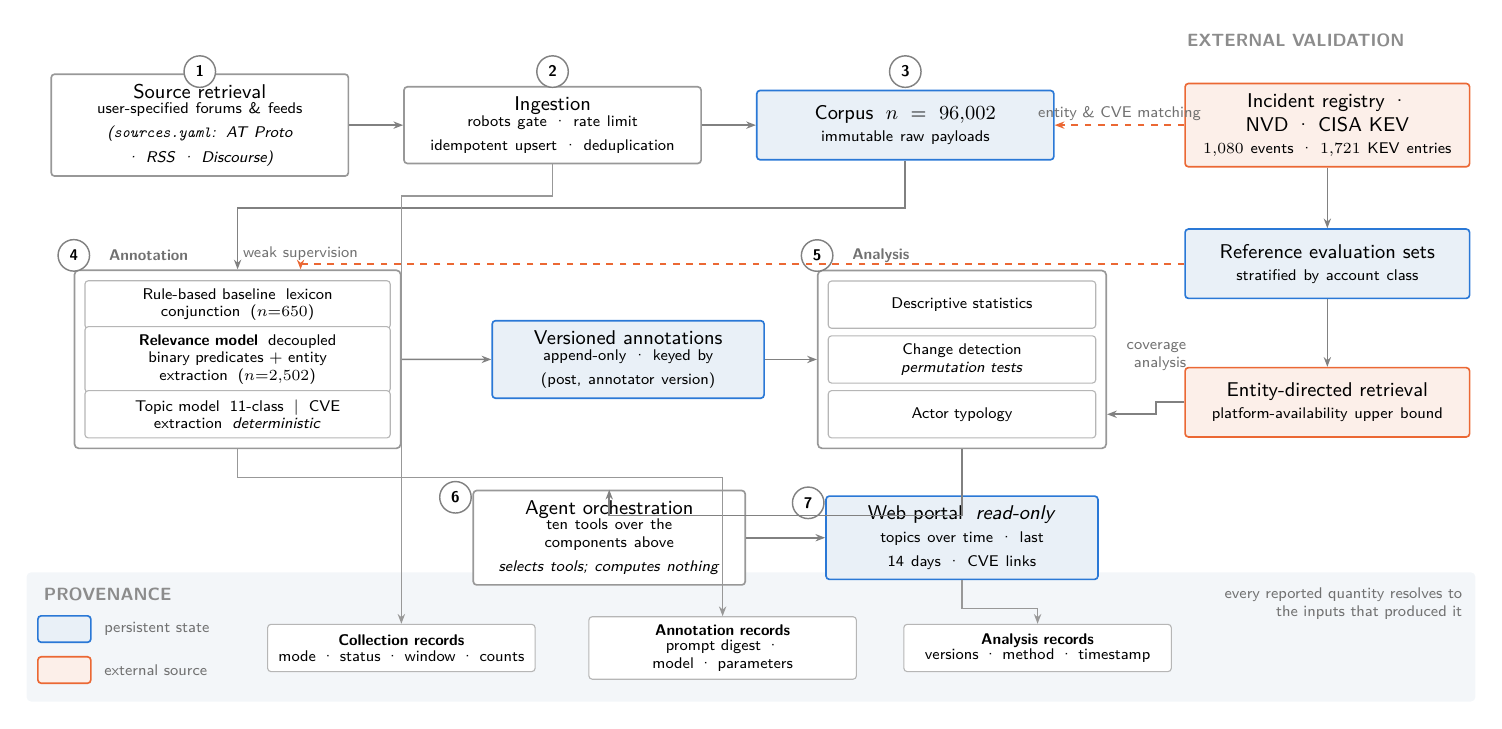
\includegraphics[width=\linewidth]{Architecture.png}
\caption{Processing pipeline. Stages 1--3 acquire and store the corpus, stage 4
annotates it under coexisting versioned schemes, stage 5 analyses the result,
and stages 6--7 expose it. The external-validation column supplies labels no
component of the pipeline produced; the provenance band records what produced
every reported quantity.}
\label{fig:arch}
\end{figure}

\section{What was built}

Collection runs in two modes against the term list --- a day-by-day backfill
and an hourly incremental --- with idempotent ingestion, stale-run reaping and
client-timestamp repair. The corpus stands at 96{,}002 posts across three
sources. Annotation proceeded in generations, all retained: two lexicon-based,
one that re-decides topic only while inheriting the relevance verdict verbatim
so that the two changes stay separately attributable, and one that replaces the
relevance decision entirely. Analysis covers descriptive statistics,
permutation testing against two null models, behavioural broadcast detection
with a collection-lag control, and a two-axis actor typology that separates
measured audience from content-judged function.

\paragraph{Sources are configuration, not code.}
\code{config/sources.yaml} names the forums and feeds to read; two generic
collectors --- RSS\slash Atom and the Discourse public JSON API --- cover most
of what a security community exposes. Both consult \code{robots.txt} and refuse
a source they cannot read, because a collector that gets blocked produces a
gap, and a gap is indistinguishable from a fall in discussion, which is the
confusion this project exists to prevent. Each source must declare why
automated access is believed permissible; the loader rejects one that does not.
Web sources reuse the existing ingest path rather than adding a second, since a
second path is a second way to bypass run bookkeeping.

\section{The collection boundary had never been examined}

The collector issues one search per term over a fixed list of 34 cybersecurity
terms --- 25 English, 9 French --- and merges the results. None of the 34
mentions Canada. The list had not changed since the first day of the project;
the \code{query\_version} mechanism faithfully recorded that it was
\code{cyber\_v1}, which guarantees reproducibility but says nothing about
adequacy.

Because platform search is close to text matching, per-term productivity can be
reconstructed offline from the stored corpus without new collection.
Figure~\ref{fig:terms} plots what each term cost against what it returned.

\begin{figure}[htbp]\centering
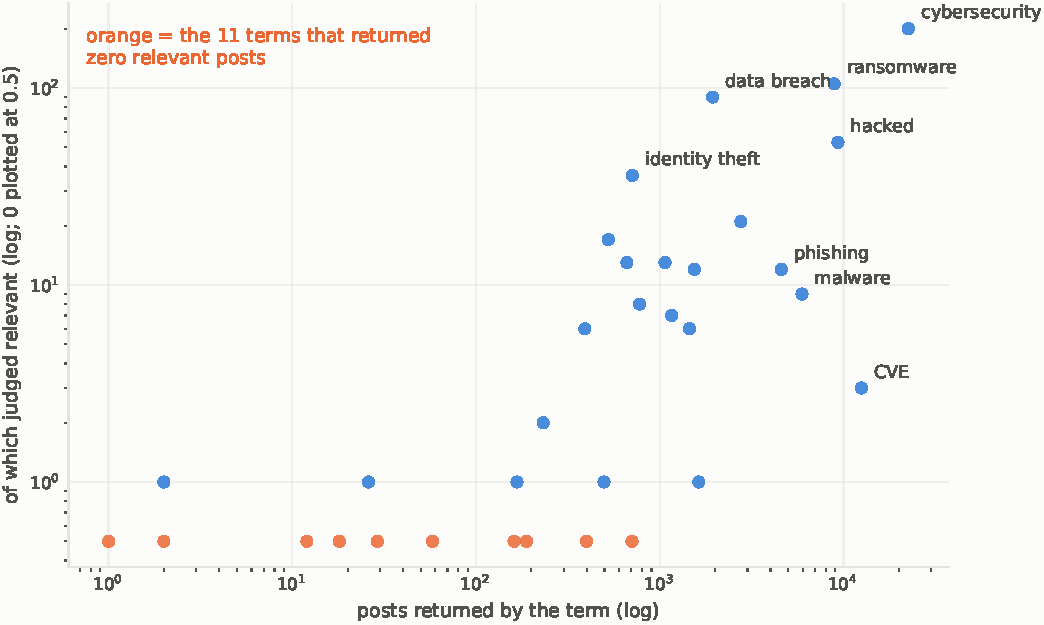
\includegraphics[width=\linewidth]{iter_terms.pdf}
\caption{Each search term: posts retrieved against posts subsequently judged
relevant. Both axes are logarithmic; terms with zero relevant posts are drawn
at $0.5$ so they remain visible. The distribution is not merely uneven --- it is
close to degenerate.}
\label{fig:terms}
\end{figure}

Three properties matter more than the ranking:

\begin{itemize}[leftmargin=1.4em,itemsep=2pt]
\item \code{CVE} retrieved 12{,}502 posts and yielded 3 relevant ones, a
      precision of $0.024\%$. It accounts for $13.7\%$ of everything collected.
\item Eleven terms returned zero relevant posts. One of them, \code{maliciel},
      returned no posts at all in 30 days.
\item \code{cybersecurity} alone accounts for $30.8\%$ of all relevant posts
      and $24.6\%$ of the entire corpus. The time series of the corpus is, to
      first order, the time series of one search term. Nothing monitored it.
\end{itemize}

\begin{warnbox}
The instructive part is the provenance of the list. The project's specification
named four term pairs and wrote ``etc.''; the remaining 26 terms were supplied
during implementation from general domain knowledge. They were never derived
from data, never compared against an external list, and never revised. The
published work that does this well does one of two things: it inherits a list
from practitioners --- Tweezers (NDSS 2025) takes its keywords from a threat
intelligence company's analysts --- or it grows one from a seed by measured
expansion. Tweezers also reports what such lists cost: comparing its own
against the earlier W2E list, more than half of the tweets it collected would
have been missed by W2E, and W2E was itself missing \code{phishing},
\code{cve} and \code{patch}. Two lists built by professionals disagreed by more
than half.
\end{warnbox}

\section{The relevance gate, replaced and then measured}

The old gate was
\code{is\_relevant = has\_cyber\_term AND has\_canada\_term AND corroborated}.
Both sides are narrow instruments joined by a conjunction, so recall is bounded
by their intersection: of 91{,}551 posts collected at the time of the
measurement, 650 passed ($0.72\%$), and the 89{,}714 rejected had never been
examined by anything semantic.

The replacement asks a model two questions, and the first design decision was
to keep them apart. A single prompt asking whether a post is about
\emph{cybersecurity in Canada} produced a $6.8\%$ pass rate on previously
rejected posts, and inspection showed why: the model had collapsed the
conjunction onto the side it knows better. The passing posts were vendor
advisories, ransomware victim listings, and a French story about the French
Ministry of Education. Asked as two independent questions, the Canadian side
passed $1.08\%$, and the passing posts began to include material that should
have been there all along --- a Quebec cabinet minister responsible for
cybersecurity, \code{.ca} law-firm domains, ``GC website'' as colloquial
shorthand for the federal government.

A second decision follows from the corpus rather than from the model: ask about
Canada first, over everything, and ask about cyber only where a Canadian entity
was found. Every post in this corpus arrived through a cybersecurity search
term, so the cyber side is nearly always true and carries little information;
the Canadian side is the rare and binding one. Running it this way also
produces an entity map of the whole corpus as a by-product --- the input to
query expansion and to event linking --- and it reduces the call count from
$2N$ to $N + \varepsilon N$.

\subsection{The gate's own failure}

The first version of the entity prompt recovered Canadian entities in only
$55.4\%$ of registry-verified positive posts and --- more diagnostically --- in
only $69.0\%$ of posts containing the literal string \emph{Canada} or
\emph{Canadian}. Specificity was excellent at $99.5\%$. The failure was
therefore recall, and its cause was the prompt: a clause instructing the model
that an empty list is the expected answer, followed by a long list of
prohibitions, drove a 4B model to the null answer. Removing the restraint
clause and adding an explicit rule --- if the country name appears literally,
it counts --- moved literal-mention recall from $69.0\%$ to $99.3\%$
(Figure~\ref{fig:prompt}).

\begin{figure}[htbp]\centering
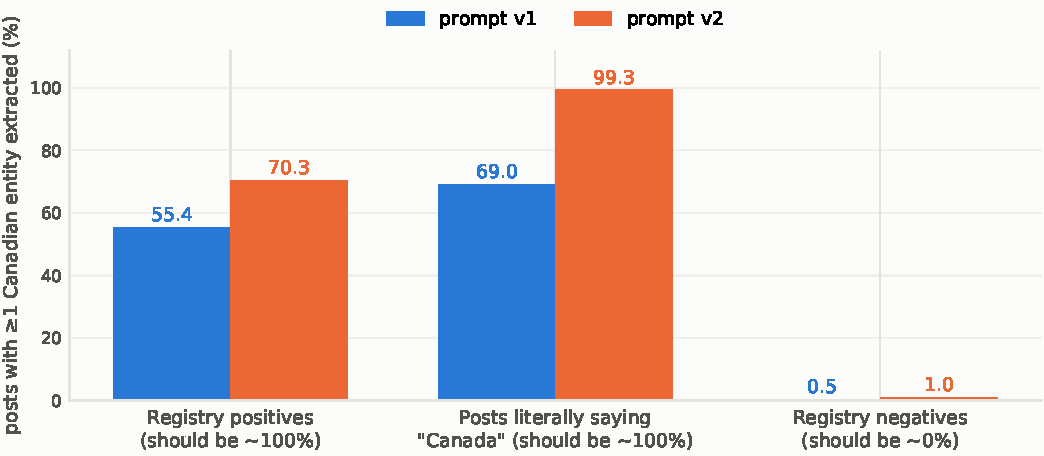
\includegraphics[width=0.82\linewidth]{iter_prompt.pdf}
\caption{Entity recall before and after the prompt revision, on posts that
contain the country name literally. The revision fixed the failure it targeted,
and introduced a second one that no evaluation set in the project could see.}
\label{fig:prompt}
\end{figure}

\subsection{And the fix broke something the evaluation could not see}

The corrected prompt raised corpus relevance from 906 posts to 3{,}528. That
number is wrong. Inspection of the additions found \code{trustedsec.com},
\code{malwarebytes.com}, the UK's \code{NCSC}, \code{Revolut}, a French story
about the \emph{\'Education nationale}, and \code{ia.cr} --- the Costa Rican
top-level domain. The prompt's clause \emph{``a \code{.ca} or \code{.gc.ca}
domain''} had been generalised by the model into \emph{``a domain''}.

Two mechanical checks, requiring no further model calls, quantify it:

\begin{center}
\begin{tabularx}{\linewidth}{@{}Lrr@{}}
\toprule
\hd{Extracted entity type} & \hd{Count} & \hd{Not present in the post text} \\
\midrule
\code{place}         & 2{,}192 & \textbf{1{,}053 \;(48.0\%)} \\
\code{org}           & 1{,}364 & 12 \;(0.9\%) \\
\code{domain}        & 1{,}296 & 49 \;(3.8\%) \\
\code{gov}           & 889     & 10 \;(1.1\%) \\
\midrule
\multicolumn{3}{@{}l}{\small Of the 1{,}296 \code{domain} entities, 312
($24.1\%$) actually end in a Canadian TLD.} \\
\bottomrule
\end{tabularx}
\end{center}

\begin{keybox}
\textbf{A verification channel obtained by accident.} Character offsets are
computed with \code{str.find} rather than requested from the model, on the
narrow grounds that small models miscount offsets. That decision turned into an
independent hallucination detector: an entity string that cannot be located in
the post was invented. Nearly half of all \code{place} entities were --- the
model writing ``Canada'' into a French post about a French ministry. Declining
to trust a model with a task it does badly produced a free check on the task it
was actually given.
\end{keybox}

Applying both rules --- discard entities absent from the text, discard domains
outside Canadian TLDs --- removes 2{,}086 entities and 1{,}180 posts. The
validation layer is retained in the labeler even though the prompt has been
corrected, because it is deterministic, costs nothing, and catches exactly the
class of error the external evaluation set cannot.

\begin{center}
\begin{tabularx}{\linewidth}{@{}Lrrr@{}}
\toprule
\hd{Relevance gate} & \hd{recall} & \hd{specificity} & \hd{corpus} \\
 & \hd{@\,registry pos.} & \hd{@\,registry neg.} & \hd{relevant} \\
\midrule
\code{rules\_v2} --- keyword conjunction       & 46.5\% & 99.8\% & 650 \\
\code{llm\_v2a} --- two questions, prompt v1   & 53.5\% & 99.7\% & 860 \\
\code{llm\_v2c} --- prompt v2 + validation     & \textbf{68.3\%} & 99.4\% & \textbf{2{,}348} \\
\midrule
\multicolumn{4}{@{}l}{\small \emph{before} validation, prompt v2 reported
$69.3\%$ / $99.0\%$ / 3{,}528 --- one third of that corpus was spurious.} \\
\bottomrule
\end{tabularx}
\end{center}

\begin{warnbox}
\textbf{The negative set certified a corpus that was a third wrong.} A
specificity of $99.0\%$ on the registry negative set implies roughly 890 false
positives across 89{,}044 posts. The true figure was 1{,}181. The negative set
did not detect the failure because it is composed of feed posts about foreign
ransomware victims: formulaic English, few URLs, no French. The model's actual
failure modes --- over-generalising a domain rule, hallucinating a country name
into French text --- do not occur in that population. An external label removes
self-reference; it does not confer representativeness, and a non-representative
evaluation set does not merely fail to detect a regression, it actively
certifies one.
\end{warnbox}

\subsection{What remains is a knowledge ceiling}

Of the posts the corrected and validated extractor still misses, \textbf{none}
contains the word \emph{Canada} in any form. They read \emph{``New post from
\#Qilin: Coldfish Seafood''} --- a real Canadian victim, named, with no country
marker anywhere in the text. No amount of prompting will let a 4B model know
that Coldfish Seafood is Canadian.

\begin{keybox}
This is a ceiling of a particular kind. The residual error in the relevance
gate is not a model-capability problem and not a prompt problem: it is missing
world knowledge about small Canadian organisations. The only thing that
resolves it is a gazetteer --- and the gazetteer that would resolve it is the
external registry currently being used to measure the gap. The measurement
instrument and the repair are the same object.
\end{keybox}

\section{An external reference, and what it revealed about itself}

Until this phase, every precision and recall figure in the project traced back
to a single author: the person who wrote the rules also wrote the prompts and
produced the hand-coded evaluation set. A reported $\kappa = 0.870$ measures
agreement under those conditions, not independence.

An incident registry breaks that loop. Victim records were ingested for Canada
(positives) and the United States, France and the United Kingdom (negative
entity sources): 1{,}080 events and 1{,}943 entities. Matching victim
organisation names against the corpus produces evaluation sets whose labels no
part of this system produced.

Two constraints were imposed on their construction, and both mattered more than
expected.

\emph{First, the definition of an evaluation set may not contain the output of
the system being evaluated.} A natural specification for the negative set was
``mentions a foreign victim, and \code{rules\_v2} judged \code{is\_canada}
false''. That specification makes \code{rules\_v2} precision identically $1$ on
the set, and any replacement can only appear worse --- an artefact of
construction with no relation to capability. The negative set uses registry
conditions only.

\emph{Second, the positive set must be stratified by account type.} The reason
is visible in the data: registry victim names appear on the platform almost
exclusively inside the accounts that syndicate the registry. Of 101 positive
posts, 100 come from automated feeds. Median engagement is zero and $94.9\%$ of
the posts have no likes at all. The single post classified as non-feed turned
out to be a golf-industry content farm auto-generating an article about a golf
club's ransomware incident, with zero likes, reposts and replies.

\begin{warnbox}
\textbf{A metric that rewards capturing bots.} Had recall on the registry
positive set been adopted as the optimisation target, it would have climbed
towards $100\%$, because those posts are formulaic and a model need only learn
which small firms are Canadian. The metric would improve substantially while
the research question --- what Canadians say about cyber incidents --- received
no answer at all. External labels are necessary but not sufficient: an external
label attached to a non-independent \emph{population} reintroduces the
circularity it was meant to remove.
\end{warnbox}

\section{The central result}

Combining the registry with a targeted per-event search over the platform
separates the three explanations. For every Canadian event in the window, the
victim organisation's name was searched directly --- with no cybersecurity term
attached --- over a $[-2, +30]$ day window. Because bare organisation names
attract unrelated traffic (\emph{Air Canada} retrieves fare deals), every hit
was then passed through the cyber judgement before counting. This is
entity-directed retrieval: it establishes an upper bound on what the platform
could have yielded for an event whose identity is already known.

\begin{figure}[htbp]\centering
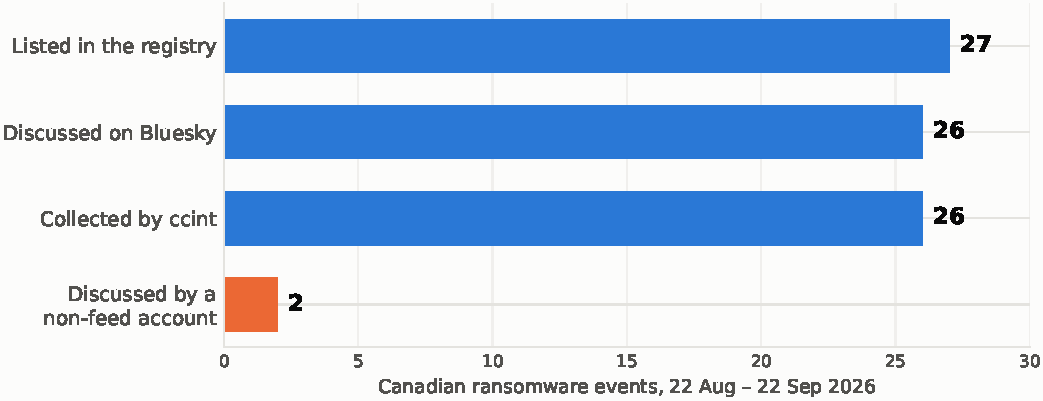
\includegraphics[width=\linewidth]{iter_funnel.pdf}
\caption{The same 27 Canadian ransomware events at four successive gates. The
attrition is almost entirely at the last one, and the last one is not a
property of this system.}
\label{fig:funnel}
\end{figure}

\begin{center}
\begin{tabularx}{\linewidth}{@{}Lrr@{}}
\toprule
\hd{Stage} & \hd{Events} & \hd{Share} \\
\midrule
Listed in the registry, in window & 27 & --- \\
At least one cyber-related post exists on the platform & 26 & 96\% \\
At least one such post was collected by ccint & 26 & 96\% \\
At least one such post came from a non-feed account & \textbf{2} & \textbf{7\%} \\
\bottomrule
\end{tabularx}
\end{center}

\medskip

The 144 cyber-related posts across these events come from 15 accounts. Twelve
are automated threat-intelligence feeds. The three that are not are Canadian
news organisations, contributing five posts between them, all about the same
event. Individual users contributed nothing.

\begin{keybox}
\textbf{The collector is not the bottleneck for this event class.} It captured
26 of the 26 events the platform carried. The reason the corpus contains no
detectable trend in ransomware discussion is that there is almost no ransomware
\emph{discussion} to detect --- there is a nearly complete mirror of several
leak-site feeds, and the corpus reproduces it faithfully. That also reframes
the power analysis: $8\times$ of this corpus is $8\times$ as much syndication,
so volume is the wrong lever.
\end{keybox}

\subsection{The one event that behaved differently}

The exception is worth stating in full, because it is the only case in the
month where the platform behaved the way the project assumed it would.

The Commission de la construction du Qu\'ebec, a provincial construction
industry regulator, was listed by the Qilin ransomware group; roughly 350{,}000
people's data was taken. This event drew genuine Canadian media coverage in
French and English: a class action filed in Quebec Superior Court, reporting on
the scale of the theft, and a radio interview with the CCQ's chief executive.

Four of those five posts are in the corpus. The one that is not reads
\emph{``Une protection pr\'eventive mise en place \`a la CCQ: \guillemotleft Je
me sens responsable \guillemotright''}. It contains no term from the 34-term
list --- \emph{protection pr\'eventive} is in no lexicon --- and so it was
unreachable. This is the collection-boundary gap at human scale: one post, one
missing phrase, a real event, a real Canadian outlet.

\subsection{Two gaps, and a reference that can only see one}

The measurements point at two distinct deficiencies, and conflating them would
be a mistake.

\begin{center}
\begin{tabularx}{\linewidth}{@{}Lp{4.4cm}p{4.4cm}@{}}
\toprule
 & \hd{Registry-verifiable events} & \hd{General Canadian cyber talk} \\
\midrule
Collection recall & 26/27 events (96\%) & unmeasured; at least 901 rejected
posts carry a Canadian entity \\
Binding constraint & \textbf{the platform has no organic discussion} &
\textbf{the Canada lexicon misses entities} \\
Fixable by better queries? & no & yes \\
Visible to the registry? & yes & no \\
\bottomrule
\end{tabularx}
\end{center}

\medskip

A full-corpus screen of the 83{,}370 rejected posts long enough to judge found
901 containing a Canadian entity; attribution shows $55.8\%$ failed because
\code{is\_canada} was false --- the lexicon missed the entity --- and
\emph{none} were blocked by the corroboration rule that a prior review had
proposed retiring. Of the 1{,}799 posts the new gate newly admits, $84.0\%$
were rejected by the Canadian side of the conjunction, against $12.2\%$ on the
cyber side and $3.7\%$ on both; in the other direction the new gate rejects 138
posts the rules had admitted. The asymmetry is the point: nearly all
recoverable recall sat behind the Canada lexicon.

But the registry cannot see that population at all. It contains ransomware
victims, so it can only score the class of discussion that ransomware feeds
dominate.

\section{Linking discussion to vulnerabilities}

CVE identifiers are extracted by regular expression rather than by a model.
Their format is fixed by MITRE, so extraction is deterministic; this is the one
table in the system whose trustworthiness is independent of annotation quality,
which is unusual here and worth stating plainly. Identifiers are then enriched
from two external sources the system cannot influence: NVD for theoretical
severity, and the CISA Known Exploited Vulnerabilities catalogue for the fact
of observed exploitation. The two are kept in separate columns and never
combined into a risk score. One is a judgement about how bad a flaw could be;
the other is an observation that somebody is using it. A combined number would
hide which half is external fact --- the same error, in a smaller form, as the
composite trend score this project rejected earlier.

\begin{figure}[htbp]\centering
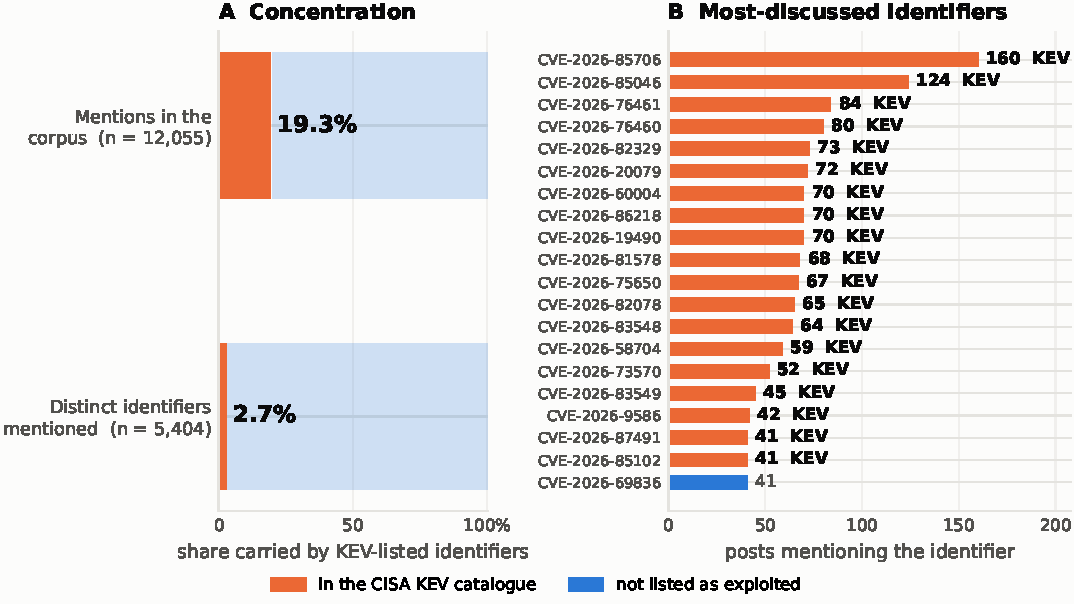
\includegraphics[width=\linewidth]{fig_cve_attention.pdf}
\caption{Attention against confirmed exploitation. \textbf{A}: identifiers in
the KEV catalogue are $2.7\%$ of those mentioned but carry $19.3\%$ of the
mentions. \textbf{B}: of the twenty most-discussed identifiers, nineteen are
KEV-listed. The two panels are deliberately separate charts --- one is a
proportion and the other a count, and a single axis carrying both would
mislead.}
\label{fig:cve}
\end{figure}

\begin{center}
\begin{tabularx}{\linewidth}{@{}Lrr@{}}
\toprule
\hd{Across the corpus, 22 Aug -- 23 Sep 2026} & \hd{Count} & \hd{Share} \\
\midrule
Posts mentioning at least one CVE identifier & 10{,}820 & --- \\
Distinct identifiers mentioned              & 5{,}404  & --- \\
Of those, listed in the CISA KEV catalogue  & 147      & 2.7\% \\
Share of all 12{,}055 mentions going to those 147 & --- & \textbf{19.3\%} \\
Of the 25 most-discussed identifiers, in KEV & \textbf{21} & 84\% \\
\bottomrule
\end{tabularx}
\end{center}

Two caveats belong with that figure. The concentration is measured over
mentions, and the feed accounts characterised above contribute a large share of
them, so this is partly a statement about what threat-intelligence syndication
prioritises. And the two enrichments are not equally complete: one catalogue
fetch covers KEV status for every identifier, whereas NVD severity is subject
to a rate limit and is currently resolved for 379 of the 5{,}404 mentioned
identifiers, prioritised by corpus prominence rather than by ease of retrieval.

\begin{keybox}[unbreakable]
\textbf{Attention tracks exploitation rather than severity.} A set of
vulnerabilities making up $2.7\%$ of those mentioned attracts $19.3\%$ of the
mentions --- a concentration of roughly sevenfold --- and more than four in five
of the most-discussed identifiers are ones CISA has independently confirmed as
exploited. This is the first result in the project where social-media attention
aligns with an external ground truth instead of mirroring a feed, and the first
that is directly usable: ranking vulnerabilities by how much they are discussed
recovers most of the confirmed-exploited set without being told what it is.
\end{keybox}

\section{Making the system answerable}

The measurements above are only useful if somebody other than their author can
interrogate them. The final layer adds no analysis. It turns the existing
components into ten tools, gives a model the ability to call them, and puts the
results behind a read-only portal.

\begin{figure}[htbp]\centering
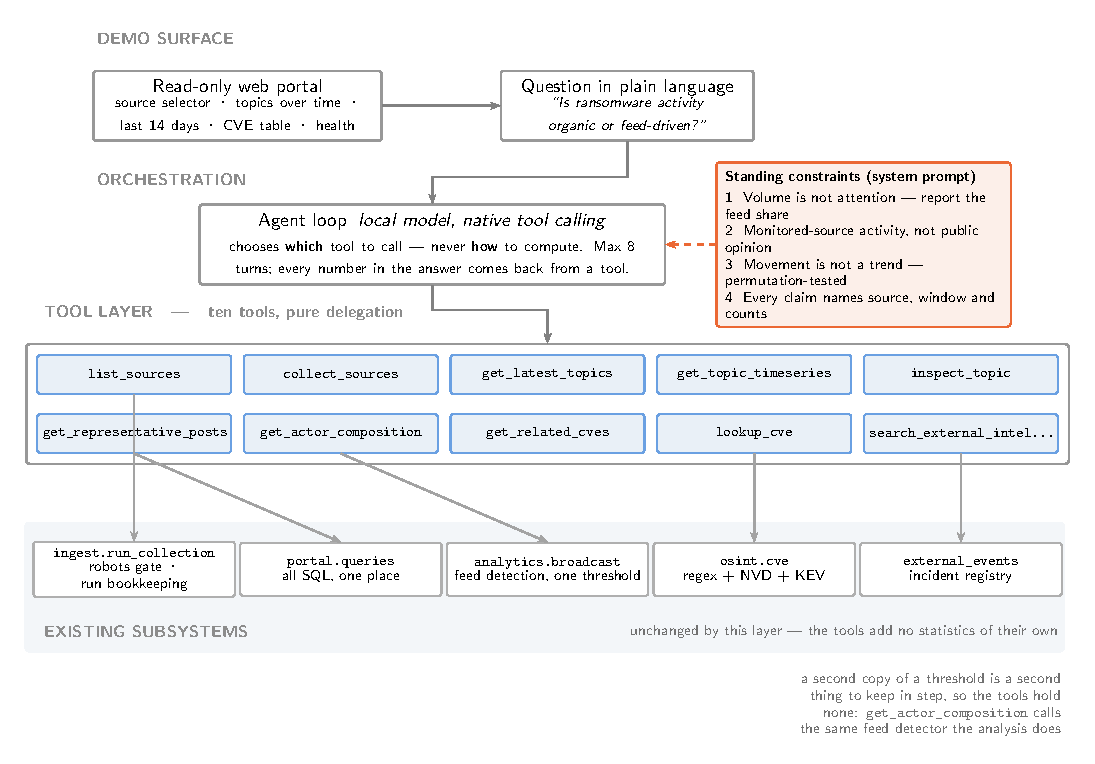
\includegraphics[width=\linewidth]{agent_stack.pdf}
\caption{The orchestration layer. The agent chooses \emph{which} tool to call;
it never chooses \emph{how} to compute. Every statistic is produced by the same
subsystem that produces it for the analysis pipeline, so a question asked twice
cannot be answered on two different definitions.}
\label{fig:agent}
\end{figure}

\paragraph{The tools compute nothing of their own.}
\code{get\_actor\_composition} forwards to the same broadcast detector the
analysis uses, with the same thresholds; \code{collect\_sources} forwards to
\code{run\_collection}, so an agent-triggered collection lands in the run
record like any other and cannot become an untracked gap; all SQL lives in one
query module. This is enforced by test rather than by convention: the suite
fails if a second copy of the broadcast threshold appears in the tool layer,
because two implementations of one definition drift apart and nobody notices
until a number is wrong in public.

\paragraph{The agent's constraints are the project's measurements.}
Four findings are written into the system prompt as standing constraints:
volume is not attention and the feed share must be reported alongside it; this
corpus describes activity in the monitored sources and not Canadian public
opinion; permutation testing found no movement distinguishable from noise, so
an increase is not a trend; and every claim must name its source, window and
counts. Severity and exploitation must be reported separately. If the backend
is unavailable the agent refuses rather than answering from memory.

Asked \emph{``Is ransomware activity mostly organic or feed-driven?''}, the
agent called \code{list\_sources}, \code{get\_latest\_topics} and
\code{inspect\_topic} across four turns and answered that activity is mostly
feed-driven, quoting the measured broadcast share, limiting the claim to the
monitored sources, and declining to describe the window-over-window change as a
trend. The interesting part is not that the model can call tools; it is that
the constraint set makes the honest answer the only one the tools support.

\paragraph{What the portal shows.}
A source selector filters every view, so a demonstration does not require
editing configuration. Beside the content it shows collection health, because a
quiet day and a broken collector look identical on a topic chart and different
in the run record. Every panel carries its own caveat text, since a bare number
on a screen reads as unconditional. Collection can be triggered only for
sources already declared in configuration; an arbitrary URL is rejected.

\begin{figure}[htbp]\centering
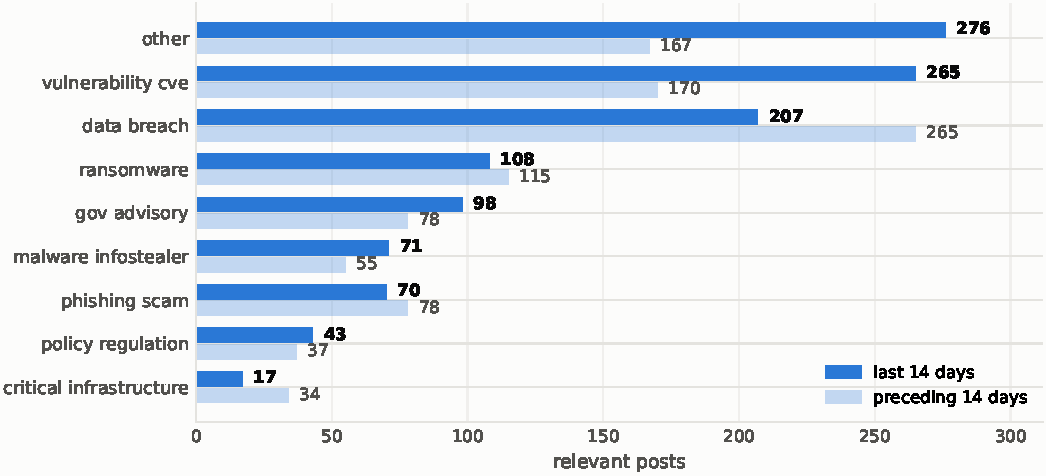
\includegraphics[width=\linewidth]{fig_recent_topics.pdf}
\caption{The last fourteen days against the preceding fourteen, as the portal
presents them. These are descriptive counts. Permutation testing on this corpus
found no topic change distinguishable from noise, so no bar here should be read
as a trend --- which is exactly why the portal labels them as activity rather
than as change.}
\label{fig:recent}
\end{figure}

Building this layer surfaced two defects in the analysis it wraps, both of the
kind that only appear when numbers are put on a screen for someone else. Topic
queries folded posts carrying no topic row into the residual \code{other}
bucket --- the same error the project had already ruled out in its actor
typology, where \code{unclassified} must never be read as a negative. Labelling
them \code{(unlabelled)} immediately exposed 962 posts in the recent window
with no topic label at all, which were then labelled. And the portal's topic
version constant still pointed at a superseded annotator, so it had been
reading a scheme covering a fraction of the corpus.

\section{What the project is}

The original framing makes a weaker claim available and a stronger one
unavailable.

Unavailable: trend analysis of Canadian cyber discourse on this platform, at
this volume, for this event class. Not because the statistics are under-powered
--- though they are --- but because the underlying signal is mostly machine
output, and adding data would add feed posts.

Available, and apparently unusual: a sensor that reports its own blind spots
with numbers. Published systems in this area report how many events they
detected --- 84 of 151 in the strongest comparable work, 45 and 4 in the
systems it compares against. All three report a numerator. None reports how
many events had no platform presence at all, because establishing that requires
the per-event entity-directed retrieval run here, and that is only affordable
when the event count is small. This project's greatest liability --- a corpus
of a few thousand relevant posts --- is exactly what makes the denominator
measurable.

\begin{keybox}
The defensible contribution is not ``we detected Canadian cyber events on
social media''. It is ``here is what a single-platform social sensor can and
cannot see about a national cybersecurity picture, measured against external
references, with the syndication component separated from the organic one, and
exposed through an interface that will not overstate it''. The first claim is
weak and partly false. The second is, as far as the surveyed literature goes,
unreported.
\end{keybox}

\section{Limitations}

\begin{itemize}[leftmargin=1.4em,itemsep=3pt]
\item \textbf{One registry, one event class.} The incident registry lists only
victims named on leak sites. Breaches disclosed by regulators, phishing
campaigns, advisories and policy events are invisible to it, as are victims who
paid. Every figure conditioned on the registry describes ransomware coverage,
not Canadian cybersecurity coverage.
\item \textbf{$N = 27$.} The three-stage decomposition rests on 27 events in
one 30-day window. The qualitative pattern is stark, but the percentages carry
wide intervals and should not be quoted as point estimates.
\item \textbf{Feed classification is a heuristic.} Accounts are labelled
automated by volume and near-zero engagement. The golf content farm shows the
failure mode: a low-volume automated account scores as organic, which biases
the organic count \emph{upward}. The true organic count is therefore no higher
than reported, and probably lower.
\item \textbf{No independent human annotation yet.} A 200-post stratified audit
sample has been drawn and deliberately left unlabelled. The person who wrote
the prompts should not be the person who scores them; doing so would reproduce
the circularity the registry was introduced to break.
\item \textbf{The evaluation sets are narrow in a way that matters.} Both are
built from ransomware victim names, so they exercise a formulaic English
subpopulation. The domain over-generalisation documented above passed them
cleanly. Any future prompt change should also be checked against a probe drawn
from the corpus itself.
\item \textbf{Multi-source collection is implemented but not demonstrated at
scale.} The two feeds added so far contributed 45 posts, because RSS exposes
only recent items and cannot be backfilled. A comparable time series requires
running them forward for weeks or adding a paginated source.
\item \textbf{A 4B model.} Both gates and the agent run on a local Qwen3-4B.
The residual gate failure --- not knowing which small firms are Canadian ---
would partly yield to a larger model, though a gazetteer addresses it more
directly and more cheaply. The agent's tool selection is reliable on the
demonstration queries but has not been evaluated systematically.
\end{itemize}

\section{What follows}

\begin{enumerate}[leftmargin=1.4em,itemsep=3pt]
\item \textbf{Widen the registry before widening anything else.} Advisories
from the Canadian Centre for Cyber Security, KEV and Canadian media would
extend the external reference past ransomware. This is the single change that
would most alter the picture above; the current denominator is narrow in a way
that flatters nothing.
\item \textbf{Feed the registry back into the gate.} The irreducible residual
is missing knowledge of Canadian organisation names, and the registry is a list
of exactly those names. This closes a loop currently open in the wrong
direction.
\item \textbf{Add a Canada-side query stream} as an additional disjunctive
stream rather than a filter --- not to improve ransomware coverage, which is
already at 96\%, but to reach the population the registry cannot see: the CCQ
interview that no cybersecurity term could retrieve.
\item \textbf{Have someone else label the audit sample.} It is the only
remaining step that cannot be automated, and the one every other number depends
on.
\item \textbf{Let the new sources accumulate,} and add a paginated one so that
multi-source comparison rests on more than 45 posts.
\item \textbf{Report absolute counts, never recall ratios.} With a denominator
this small and this biased, a ratio invites a comparison the data cannot
support.
\end{enumerate}

\vfill
\begin{plainbox}
\footnotesize
\textbf{Provenance.} The corpus stands at 96{,}002 posts across three sources,
22 August -- 23 September 2026. Gate evaluation figures were measured on 22
September against a corpus of 91{,}551 posts and are left at the values
recorded then; the incident registry and the KEV catalogue were retrieved
22--23 September. Eight annotator versions coexist over the corpus; every
model-produced label carries the SHA-256 of the prompt that produced it. The
test suite stands at 268 passing. Evaluation sets are distributed as post
identifiers with labels, not as post text.
\end{plainbox}

\end{document}
